\begin{TP}[Dominos en fractions]


Vous allez créer un jeu de dominos utilisant des fractions.

\begin{enumerate}
    \item Répartissez-vous le travail pour compléter le tableau ci-dessous. La première ligne (cases A1 à F1) contient les résultats des calculs situés dans les lignes 2 à 7.

\vspace{1em}
\renewcommand*\tabularxcolumn[1]{>{\centering\arraybackslash}m{#1}}
\renewcommand{\arraystretch}{1.6}
\begin{cltableau}{\linewidth}{7}
\hline
 & A & B & C & D & E & F \\ \hline
1 & $\dfrac{5}{3}$ & $\dfrac{-3}{5}$ & $\dfrac{3}{5}$ & $\dfrac{-9}{4}$ & $\dfrac{2}{7}$ & $3$ \\ \hline
2 & $\dfrac{1}{3} + \dfrac{4}{3}$ & $\dfrac{-4}{5} +\dfrac{1}{5}$ & & & & \\ \hline
3 & $\dfrac{7}{3}-\dfrac{4}{6}$ & $\dfrac{2}{15}-\dfrac{1}{5}-\dfrac{8}{15}$ & & & & \\ \hline
4 & $\dfrac{2}{3}+1$ & $\dfrac{12}{5}-3$ & & & & \\ \hline
5 & & & & & & \\ \hline
6 & & & & & & \\ \hline
7 & & & & & & \\ \hline
\end{cltableau}

\vspace{1em}

Quelques exemples (cases A2, B2, A3, B3, A4, B4) ont été donnés à titre indicatif. Pour chaque colonne, il faut trouver :
\begin{itemize}
    \item ligne 2 : une somme algébrique de fractions de même dénominateur ;
    \item ligne 3 : une somme algébrique de fractions de dénominateurs différents ;
    \item ligne 4 : une somme algébrique d'un nombre entier et d'une fraction ;
    \item ligne 5 : un produit de deux fractions ;
    \item ligne 6 : un produit de trois fractions ;
    \item ligne 7 : un quotient de deux fractions.
\end{itemize}

    \item Créez le jeu de dominos en respectant le plan suivant (à chaque fois, il faut remplacer le nom de la case par son contenu).
    
    Taille d'un domino : 6\,cm sur 2\,cm.
    
    \vspace{1em}
    \begin{center}
        \renewcommand*\tabularxcolumn[1]{>{\centering\arraybackslash}m{#1}}
        \begin{tabularx}{.6\linewidth}{|X|X|X|X|X|X|X|X|}
        \cline{1-2} \cline{4-5} \cline{7-8}
            A1 & A2 & & A3 & B1 & & A4 & C2 \\ \cline{1-2} \cline{4-5} \cline{7-8}
        \end{tabularx}
        \vspace{.5em}
        
        \begin{tabularx}{.6\linewidth}{|X|X|X|X|X|X|X|X|}
        \cline{1-2} \cline{4-5} \cline{7-8}
            A5 & D3 & & A6 & E4 & & A7 & F5 \\ \cline{1-2} \cline{4-5} \cline{7-8}
        \end{tabularx}
        \vspace{.5em}
        
        \begin{tabularx}{.6\linewidth}{|X|X|X|X|X|X|X|X|}
        \cline{1-2} \cline{4-5} \cline{7-8}
            B2 & B3 & & B4 & C1 & & B5 & D2 \\ \cline{1-2} \cline{4-5} \cline{7-8}
        \end{tabularx}
        \vspace{.5em}
        
        \begin{tabularx}{.6\linewidth}{|X|X|X|X|X|X|X|X|}
        \cline{1-2} \cline{4-5} \cline{7-8}
            B6 & E3 & & B7 & F4 & & C3 & C4 \\ \cline{1-2} \cline{4-5} \cline{7-8}
        \end{tabularx}
        \vspace{.5em}
        
        \begin{tabularx}{.6\linewidth}{|X|X|X|X|X|X|X|X|}
        \cline{1-2} \cline{4-5} \cline{7-8}
            C5 & D1 & & C6 & E2 & & C7 & F3 \\ \cline{1-2} \cline{4-5} \cline{7-8}
        \end{tabularx}
        \vspace{.5em}
        
        \begin{tabularx}{.6\linewidth}{|X|X|X|X|X|X|X|X|}
        \cline{1-2} \cline{4-5} \cline{7-8}
            D4 & D5 & & D6 & E1 & & D7 & F2 \\ \cline{1-2} \cline{4-5} \cline{7-8}
        \end{tabularx}
        \vspace{.5em}
        
        \begin{tabularx}{.6\linewidth}{|X|X|X|X|X|X|X|X|}
        \cline{1-2} \cline{4-5} \cline{7-8}
            E5 & E6 & & E7 & F1 & & F6 & F7 \\ \cline{1-2} \cline{4-5} \cline{7-8}
        \end{tabularx}
    \end{center}
    
    \item Découpez les dominos et échangez votre jeu avec un autre groupe. Il ne vous reste plus qu'à jouer en accolant deux cases de même valeur.
\end{enumerate}
\end{TP}

\begin{TP}[Fractions en tableur]

\begin{enumerate}
    \item Calculez puis donnez le résultat sous forme d'une fraction la plus simple possible :
    \[ A = \dfrac{-3}{7} \times \dfrac{5}{2} ; \qquad	B = \dfrac{2}{3} \times \dfrac{9}{2} \]
    \[ C = \dfrac{2}{3} + \dfrac{3}{4} ; \qquad    D = \dfrac{5}{6} + \dfrac{3}{8} \]
    \item Vous allez créer un modèle de fichier tableur permettant de trouver le produit de deux fractions :
    
    \begin{center}
        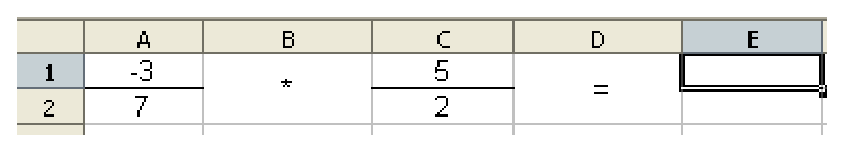
\includegraphics[width=.6\linewidth]{tableur1}
    \end{center}
    
    \begin{itemize}
        \item Recopiez les cellules ci-dessus ;
        \item Dans la cellule E1, tapez « \texttt{=A1*C1} » ;
        \item Dans la cellule E2, tapez « \texttt{=A2*C2} » ;
        \item Utilisez cette feuille de calcul pour vérifier le résultat du calcul B (question a.). Que remarquez-vous ?
    \end{itemize}
    
    \item Sur le même fichier, vous allez maintenant construire un outil permettant de calculer la somme de deux fractions.
    
    \begin{center}
        \includegraphics[width=.6\linewidth]{tableur2}
    \end{center}
    
    Recopiez les cellules ci-dessus ;
    Que faut-il taper comme formules dans les cellules E4 et E5 ?
    Utilisez cette feuille de calcul pour vérifier le résultat du calcul D (question a.). Que remarquez-vous ?
    \item Procédez de la même façon pour construire sur le même fichier quatre outils permettant :
    \begin{itemize}
        \item de calculer le produit de trois fractions ;
        \item de calculer la différence de deux fractions ;
        \item de calculer la somme de trois fractions ;
        \item de calculer le quotient de deux fractions.
    \end{itemize}
    \item Construisez un nouvel outil permettant de calculer la somme de deux fractions en faisant apparaître les étapes intermédiaires.
    \item Refaites tous les calculs avec le fichier tableur qui se trouve en complément. Quelle est la nouveauté apportée par ce fichier par rapport au vôtre ?
    \item Dans quels cas, les deux fichiers donnent-ils des résultats identiques ?
\end{enumerate}
\end{TP}